
\documentclass[12pt]{article}
\usepackage{amsmath}
\usepackage{booktabs}
\usepackage{graphicx}

% Add a front page named as Food project
\begin{titlepage}
    \begin{center}
        \vspace*{1cm}
        
        \Huge
        \textbf{Food Stastistics of College Students}
        
        \vspace{0.5cm}
        \LARGE
        \subtitle{MA4240 - Applied Statistics}
        
        \date{\today}
        
        \vspace{1.5cm}
        
        \includegraphics[width=0.4\textwidth]{your-logo}
        
        \vfill
        
        \Large
        Your Name\\
        \date{\today}
        
    \end{center}
\end{titlepage}

% Table of Contents
\tableofcontents
\newpage

\begin{document}
\section{Introduction}
{Overview }
The project tries to estimate the number of people based on many subparts that could be obtained from questions like the proportion of vegetarians and nonvegetarians in campus, Cuisine preference ratios, etc.\\
It also tries to estimate money spent by people on campus and some factors that might affect the money spent like their ability to experiment with new foods, number of dine-out days, etc.\\
On an overlook of this, we try to estimate population ratios for each type in the confidence intervals part while trying to test some hypotheses that seem general and we try to estimate where the hypotheses are true or not .\\


{Survey Questions}
These are the survey questions that were used to collect the data for project
        \begin{enumerate}
            \item Gender
            \item Type
            \item Place of Origin
            \item Which type of taste do you generally prefer in your food?
            \item Which Indian cuisine do you like the most?
            \item Which cuisine do you like to eat among foreign cuisines?
            \item How adventurous are you when it comes to trying new foods? (On a scale of 0 to 10)
            \item How often do you dine out in a typical week?
            \item On average, how much do you spend on food per month, considering dining out and other related expenses?
            \item Do you prefer having dessert after a meal, and if so, what type of dessert do you typically enjoy?
        \end{enumerate}

\section{Preprocessing of data}
The following are the steps taken for the preprocessing of data:
\begin{itemize}
    \item We started by removing white spaces and some symbols like the rupee symbol from the cost.
    \item we one hot encoded multiple options like the taste and foreign cuisine preferences for further calculations.
    eg:[Spicy, Umami] - [1,0,0,0,1]
    \item From collected as northeast Indians are fewer we classified them into north India
\end{itemize}
\section{Data Analysis}
\subsection{Observing Amount spent by each person}
In our data, we collected about the amount and various preferences. We talk about the amount spent by them and the population preferences

Here are the statistics  about the amount spent:
\begin{table}[htbp]
  \centering
  \caption{Descriptive Statistics for amount spent}
  \label{tab:stats}
  \begin{tabular}{@{}lc@{}}
    \toprule
    \textbf{Statistic} & \textbf{Value} \\
    \midrule
    Count & 223 \\
    Mean & 2350.39 \\
    Standard Deviation & 1561.59 \\
    Minimum & 529 \\
    25th Percentile & 1123 \\
    Median & 2058 \\
    75th Percentile & 2909.5 \\
    Maximum & 6951 \\
    \bottomrule
  \end{tabular}
\end{table}
\begin{figure}[htbp]
  \centering
  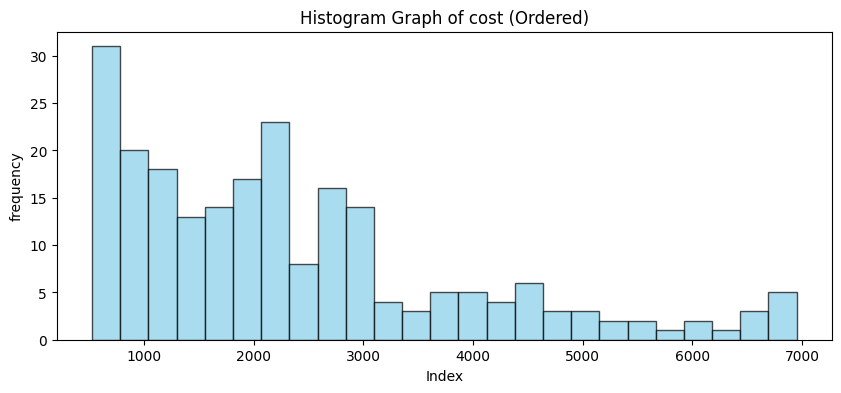
\includegraphics[width=1.0\textwidth]{Histogram for amount spent.png} % Replace 'example-image' with your image filename
  \caption{Histogram for amount spent}
  \label{fig:histogram}
\end{figure}
 \\It is left skewed gaussian.
 \\
 \\
 \newpage
 \subsection{Observing the Level of Adventurousness and its Proportion of Data}

\begin{figure}[htbp]
    \centering
    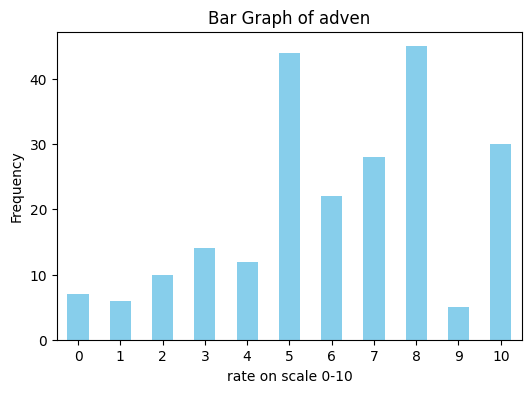
\includegraphics[width=1\textwidth]{output_57_0.png} % Change to your image filename
    \caption{Bar Graph on Adventurous Level} % Caption for the image
    \label{fig:Dessert_Preferences_1} % Label to refer to the image in the text
\end{figure}

\begin{figure}[htbp]
    \centering
    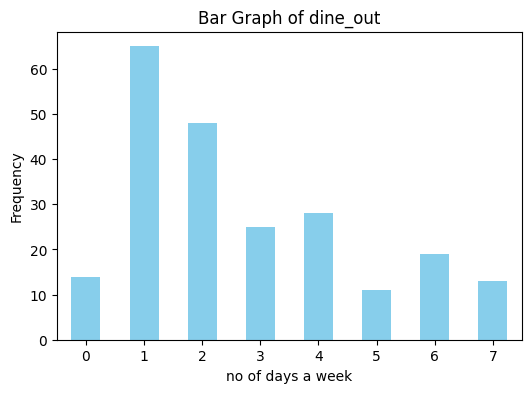
\includegraphics[width=1\textwidth]{output_65_0.png} % Change to your image filename
    \caption{Bar Graph on Dine Out} % Caption for the image
    \label{fig:Dessert_Preferences_2} % Label to refer to the image in the text
\end{figure}

 \\
 By observing the graphs we can infer the number of people and their tendency to experiment with food .
 \begin{table}[htbp]
  \centering
  \caption{Descriptive Statistics for level of adventurous}
  \label{tab:stats}
  \begin{tabular}{@{}lc@{}}
    \toprule
    \textbf{Statistic} & \textbf{Value} \\
    \midrule
    Count & 223 \\
    Mean & 6.14 \\
    Standard Deviation & 2.61 \\
    Minimum & 0 \\
    25th Percentile & 5 \\
    Median & 6 \\
    75th Percentile & 8 \\
    Maximum & 10 \\
    \bottomrule
  \end{tabular}
\end{table}
 \\This is later used to estimate money spent on food and their respective level of adventurousness 

 \subsection{observing  dineout frequencies per week.}
 Statistics obsvered for this:
 \begin{table}[htbp]
  \centering
  \caption{Descriptive Statistics for dine-out frequency}
  \label{tab:stats}
  \begin{tabular}{@{}lc@{}}
    \toprule
    \textbf{Statistic} & \textbf{Value} \\
    \midrule
    Count & 223 \\
    Mean & 2.73 \\
    Standard Deviation & 1.98 \\
    Minimum & 0 \\
    25th Percentile & 1 \\
    Median & 2 \\
    75th Percentile & 4 \\
    Maximum & 7 \\
    \bottomrule
  \end{tabular}
\end{table}


 This is later used to estimate average number of days average person of campus eats out.
\section{Confidence Intervals} 
\subsection{Type of Diet}


 This section speaks about the proportions of our survivors that prefer vegetarian and non-vegetarian.
    
    The following are stats related to it.
    
    Let $\pi_1$ denote the proportion of Vegetarians and $\pi_2$ denote the proportion of Non-Vegetarians.
    \begin{align}
        &\text{No. of Vegetarians, } n_{\text{V}} = 79 \\
        &\text{No. of Non-Vegetarians, } n_{\text{NV}} = 144 
    \end{align}

    \begin{equation}
        \hat{\pi}_1 = \frac{n_{\text{V}}}{n_{\text{V}} + n_{\text{NV}}} = 0.35, \quad \hat{\pi}_2 = \frac{n_{\text{NV}}}{n_{\text{V}} + n_{\text{NV}} } = 0.65
    \end{equation}


\subsubsection{Confidence Interval for Ratio of vegetarians}

    The following formula can be used to calculate the confidence interval of the fraction  of vegetarians 
    \begin{equation}
    \hat{\pi}_1 \pm z_{\frac{\alpha}{2}} \sqrt{\frac{\hat{\pi}_1(1 - \hat{\pi}_1)}{n}}
    \end{equation}
    By substituting, we get,
    \begin{equation}
    0.35 \pm 1.96 \times \sqrt{\frac{0.35(1 - 0.35)}{223}}
    \end{equation}
    
    i.e.,

    \[
    0.35 \pm 0.062 = (0.291, 0.417)
    \]

    
    Thus, we can be 95\% confident that between the ratio of 0.291 and 0.417 of the population on the campus prefers vegetarianism.

\subsubsection{Confidence Interval for Ratio of vegetarians}

    Similarly, by using the same formula, we can calculate the CI for the fraction of non-vegetarians as
    \begin{equation}
    \hat{\pi}_2 \pm z_{\frac{\alpha}{2}} \sqrt{\frac{\hat{\pi}_2(1 - \hat{\pi}_2)}{n}}
    \end{equation}
    Substituting the values, we get
    \begin{equation}
    0.65 \pm 1.96 \times \sqrt{\frac{0.65(1 - 0.65)}{223}}
    \end{equation}
    
    i.e.,

    \[
    0.65 \pm 0.062 = (0.582, 0.708)
    \]

    
    Thus, we can be 95\% confident that between the ratio of 0.582 and 0.708 the population on the campus prefer Non-vegetarian.


\subsection{Taste Preferences}


 This section speaks about the proportions of our survey related to their taste preferences
    
    The following are stats related to it.
    
    Let $\pi_1$ denote the proportion of people who prefer sweet and $\pi_2$ denote the proportion of people who prefer salt...
    \begin{align}
        &\text{No. of that prefer sweet taste, } n_{\text{1}} = 93 \\
        &\text{No. of that prefer salty taste, } n_{\text{2}} = 54 \\
        &\text{No. of that prefer sour taste, } n_{\text{3}} = 44\\
        &\text{No. of that prefer spicy taste, } n_{\text{4}} = 176 \\
        &\text{No. of that prefer umami taste, } n_{\text{5}} = 21\\
        &\text{No. of people, } n_{\text{T}} = 223
    \end{align}
    So,
    \begin{equation}
        \hat{\pi}_1  = 0.42, \quad \hat{\pi}_2  = 0.25, \quad \hat{\pi}_3  = 0.2, \quad \hat{\pi}_4  = 0.79, \quad \hat{\pi}_5  = 0.09
    \end{equation}
  Now,
  For large random samples, a $100(1 - \alpha)\%$ confidence interval for population proportion $p_i$ is:

    
    
    \[
    \hat{p}i \pm z_{\frac{\alpha}{2}} \sqrt{\frac{\hat{p}_i(1 - \hat{p}_i)}{n}}
    \quad \text{for } i = 1, 2, 3, 4
    \]
\subsubsection{Confidence Intervals}
    On applying the above formula we get the following confidence intervals
    \begin{itemize}
        \item Thus, we can be 95\% confident that between the ratio of 0.352 and 0.482, the population on the campus prefers sweet flavour.
        
        \item Thus, we can be 95\% confident that between the ratio of 0.19 and 0.303, the population on the campus prefers Salty flavor.
        
        \item Thus, we can be 95\% confident that between the ratio of 0.145 and 0.303, the population on the campus prefers Sour flavor.
        
        \item Thus, we can be 95\% confident that between the ratio of 0.736 and 0.843, the population on the campus prefers Spicy flavor.
        
        \item Thus, we can be 95\% confident that between the ratio of 0.056 and 0.133, the population on the campus prefers Umami Flavor.
    \end{itemize}


\subsection{Cuisine preferences }
 This section speaks about surveyors and their foreign cuisine preferences.
    
    The following are stats related to it.
    
    Let $\pi_1$ denote the proportion of people who prefer sweet and $\pi_2$ denote the proportion of people who prefer salt...
    \begin{align}
        &\text{No. of that prefer Japanese cuisine, } n_{\text{1}} = 63 \\
        &\text{No. of that prefer Italian cuisine, } n_{\text{2}} = 115 \\
        &\text{No. of that prefer Chinese cuisine, } n_{\text{3}} = 135\\
        &\text{No. of that prefer Mexican cuisine, } n_{\text{4}} = 60\\
        &\text{No. of people, } n_{\text{T}} = 223
    \end{align}
    So,
    \begin{equation}
        \hat{\pi}_1  = 0.28, \quad \hat{\pi}_2  = 0.52, \quad \hat{\pi}_3  = 0.60, \quad \hat{\pi}_4  = 0.27
    \end{equation}
  Now,
  For large random samples, a $100(1 - \alpha)\%$ confidence interval for population proportion $p_i$ is:
    
    \[
    \hat{p}i \pm z_{\frac{\alpha}{2}} \sqrt{\frac{\hat{p}_i(1 - \hat{p}_i)}{n}}
    \quad \text{for } i = 1, 2, 3, 4
    \]
\subsubsection{Confidence Intervals}
    On applying the above formula we get the following confidence intervals
    \begin{itemize}
         \item Thus, we can be 95\% confident that between the ratio of 0.223 and 0.342, the population on the campus prefers Japanese cuisine.
        
        \item Thus, we can be 95\% confident that between the ratio of 0.45 and 0.581, the population on the campus prefers Italian cuisine.
        
        \item Thus, we can be 95\% confident that between the ratio of 0.541 and 0.67, the population on the campus prefers Chinese cuisine.
        
        \item Thus, we can be 95\% confident that between the ratio of 0.211 and 0.327, the population on the campus prefers Mexican cuisine.
    \end{itemize}


\subsection{Dessert preferences}
    This subsection speaks about  our surveyors and Their frequency of desert consumption 
    
    The following are stats related to it.
    
    Let $\pi_1$ denote the proportion of people who prefer sweet and $\pi_2$ denote the proportion of people who prefer salt...
    \begin{align}
        &\text{No. of people that prefer dessert often , } n_{\text{1}} = 81 \\
        &\text{No. of people that prefer dessert rarely , } n_{\text{2}} = 116 \\
        &\text{No. of people that do not prefer dessert, } n_{\text{3}} = 26\\
        &\text{No. of people, } n_{\text{T}} = 223
    \end{align}
    So,
    \begin{equation}
        \hat{\pi}_1  = 0.36, \quad \hat{\pi}_2  = 0.52, \quad \hat{\pi}_3  = 0.12
    \end{equation}
  Now,
  For large random samples, a $100(1 - \alpha)\%$ confidence interval for population proportion $p_i$ is:
    
    \[
    \hat{p}i \pm z_{\frac{\alpha}{2}} \sqrt{\frac{\hat{p}_i(1 - \hat{p}_i)}{n}}
    \quad \text{for } i = 1, 2, 3, 4
    \]
\subsubsection{Confidence Intervals}
    On applying the above formula we get the following confidence intervals
    \begin{itemize}
        \item We can be  95\% confident that between the ratio of \textbf{0.3 and 0.426}, the population on the campus prefers Dessert \textbf{Often}.
        
        \item We can be  95\% confident that between the ratio of \textbf{0.455 and 0.586}, the population on the campus prefers Dessert \textbf{rarely}.
        
        \item Thus, we can be  95\% confident that between the ratio of \textbf{0.074 and 0.159}, the population on the campus \textbf{does not prefer} having Dessert.
    \end{itemize}

\subsection{Cost statistics : Confidence Intervals for the amount spent by different adventurous level people}
In this section, we examine expenditure patterns across different levels of adventurousness among individuals. Confidence intervals were calculated to estimate mean expenditures for each category

     \\ If $X_1, X_2, \ldots, X_n$ are normally distributed with unknown mean $\mu$ and variance $\sigma^2$, then a $(1 - \alpha) \times 100\%$ confidence interval for the population mean $\mu$ is:

        \[
        \bar{x} \pm t_{\frac{\alpha}{2}, n-1} \frac{S}{\sqrt{n}}
        \]
    \subsubsection{Confidence Intervals for the amount spent by low adventurous level people}
        The central tendencies are as follows:
        \begin{itemize}
            \item \textbf{Count} n:23.000000.
            \item \textbf{Mean} $\bar{x}$ : 2898.782609.
            \item \textbf{Std} S: 1967.060519
            \item \textbf{Min}: 564.000000.
            \item \textbf{25\%}: 1152.000000.
            \item \textbf{50\%}: 2267.000000.
            \item \textbf{75\%}: 4731.000000.
            \item \textbf{Max}: 6627.000000.
        \end{itemize}

         Using the following formula we get CI with confidence 95\% as
        \begin{equation}
        \bar{x} \pm t_{\frac{\alpha}{2}, n-1} \frac{S}{\sqrt{n}} =
        2898.78 \pm 2.07 \frac{1967.06}{\sqrt{23}}  = (2048.161,3749.403)
        \end{equation}

        From the respective calculations, we can see that:
        
        \item The mean of money spent by people that fall into the category of \textbf{low adventurous level} will lie in the interval \textbf{(2048.161, 3749.403)} with a confidence of \textbf{95\%}.
        
    \subsubsection{Confidence Intervals for amount spent by medium adventurous level people}
        The central tendencies are as follows:
        \begin{itemize}
            \item \textbf{Count} n:70.000000.
            \item \textbf{Mean} $\bar{x}$ : 2283.928571.
            \item \textbf{Std} S: 1430.839931
            \item \textbf{Min}: 587.000000.
            \item \textbf{25\%}: 1141.500000.
            \item \textbf{50\%}: 2056.000000.
            \item \textbf{75\%}: 2692.000000.
            \item \textbf{Max}: 6890.000000.
        \end{itemize}

        Using the following formula we get CI with confidence 95\% as
        \begin{equation}
        \bar{x} \pm t_{\frac{\alpha}{2}, n-1} \frac{S}{\sqrt{n}} =
        2283.92 \pm 1.99 \frac{1430.83}{\sqrt{70}} = (1942.757,2625.100)
        \end{equation}

        From the respective calculations, we can see that:
        \item The mean of money spent by people that fall into the category of \textbf{mid-adventurous level} will lie in the interval \textbf{(1942.757, 2625.100)} with a confidence of \textbf{95\%}.
    
    \subsubsection{Confidence Intervals for amount spent by high adventurous level people}
        The central tendencies are as follows:
        \begin{itemize}
            \item \textbf{Count} n:95.000000.
            \item \textbf{Mean} $\bar{x}$ : 2271.831579.
            \item \textbf{Std} S: 1435.554846
            \item \textbf{Min}: 513.000000.
            \item \textbf{25\%}: 1086.000000.
            \item \textbf{50\%}: 1935.000000.
            \item \textbf{75\%}: 2963.000000.
            \item \textbf{Max}: 6900.000000.
        \end{itemize}

        Using the following formula, we get CI with confidence 95\% as
        \begin{equation}
        \bar{x} \pm t_{\frac{\alpha}{2}, n-1} \frac{S}{\sqrt{n}} =
        2271.83 \pm 1.985 \frac{1435.55}{\sqrt{95}}  = (1979.394,2564.269)
        \end{equation}

         From the respective calculations, we can see that:
         \item The mean of money spent by people that fall into the category of \textbf{high adventurous level} will lie in the interval \textbf{(1979.394, 2564.269)} with a confidence of \textbf{95\%}.
        
    
    \subsubsection{Confidence Intervals for amount spent by very high adventurous level people}
         The central tendencies are as follows:
        \begin{itemize}
            \item \textbf{Count} n:35.000000
            \item \textbf{Mean} $\bar{x}$ : 2191.400000.
            \item \textbf{Std} S: 1397.002931
            \item \textbf{Min}: 549.000000.
            \item \textbf{25\%}: 934.500000.
            \item \textbf{50\%}: 2161.000000.
            \item \textbf{75\%}: 2638.000000.
            \item \textbf{Max}: 5263.000000.
        \end{itemize}
         Using the following formula, we get CI with confidence 95\% as
        \begin{equation}
        \bar{x} \pm t_{\frac{\alpha}{2}, n-1} \frac{S}{\sqrt{n}} =
        2191.40 \pm 2.032 \frac{1397.0}{\sqrt{35}} = (1722.545,2660.255)
        \end{equation}

        From the respective calculations, we can see that:
        
        \item The mean of money spent by people that fall into the category of \textbf{very high adventurous level} will lie in the interval \textbf{(1722.545, 2660.255)} with a confidence of \textbf{95\%}.

\subsection{Confidence Interval for the number of days the students  dine out per week}
    This part studies the number of days the students of our campus dine out per week. 

        \begin{itemize}
            \item \textbf{Count} n:223.000000
            \item \textbf{Mean} $\bar{x}$ : 2.726457.
            \item \textbf{Std} S: 1.977707
            \item \textbf{Min}: 0.000000.
            \item \textbf{25\%}: 1.000000.
            \item \textbf{50\%}: 2.000000.
            \item \textbf{75\%}: 4.000000.
            \item \textbf{Max}: 7.000000.
        \end{itemize}
    \\
    Using the following formula, we get CI with confidence 95\% as
        \begin{equation}
        \bar{x} \pm t_{\frac{\alpha}{2}, n-1} \frac{S}{\sqrt{n}} =
        2.73 \pm 1.970 \frac{1.977}{\sqrt{223}} = (2.465,2.987)
        \end{equation}
    Thus, the average number of days of dining out of our campus students falls in the interval (2.465,2.987) with a confidence of 95\%  

\section{Hypothesis Testing:}
    \subsection{Hypothesis -1}
       \textbf{Hypothesis:}
        The proportion of vegetarians who prefer dessert after meals is higher than the proportion of non-vegetarians who prefer dessert after meals
       \medskip
       
    Let $\pi_1$ denote the proportion of Vegetarians preferring dessert after meals and $\pi_2$ denote the proportion of Non-Vegetarians preferring dessert after meals.
    \begin{align}
        &\text{No. of Vegetarians in sampled data, } n_{\text{V}} = 49 \\
        &\text{No. of Non-Vegetarians in sampled data, } n_{\text{NV}} = 100 \\
        &\text{No. of Vegetarians preferring dessert, } n_{\text{Vp}} = 23 \\
        &\text{No. of Non-Vegetarians preferring dessert, } n_{\text{NVp}} = 30
    \end{align}
    So,
    \begin{equation}
        \hat{\pi}_1 = \frac{n_{\text{Vp}}}{n_{\text{V}}} = 0.47, \quad \hat{\pi}_2 = \frac{n_{\text{NVp}}}{n_{\text{NV}}} = 0.30
    \end{equation}

    Now,
    \begin{align}
        H_0 &: \pi_1 - \pi_2 \leq 0 \\
        H_a &: \pi_1 - \pi_2 > 0
    \end{align}
    Now, we check the conditions:
    \begin{align}
        n_1\hat{\pi}_1 &\geq 5, \quad n_1(1 - \hat{\pi}_1) \geq 5 \\
        n_2\hat{\pi}_2 &\geq 5, \quad n_2(1 - \hat{\pi}_2) \geq 5
    \end{align}
    So, the test statistic is
    \begin{equation}
        Z = \frac{\hat{\pi}_1 - \hat{\pi}_2}{\sqrt{\frac{\hat{\pi}_1(1-\hat{\pi}_1)}{n_1} + \frac{\hat{\pi}_2(1-\hat{\pi}_2)}{n_2}}} = 2.00
    \end{equation}
    and
    \begin{equation}
        z_{0.05} = 1.645
    \end{equation}
     \medskip
     
    \textbf{Rejection Region approach:}
We will reject $H_0$ if the test statistic $Z > Z_{\alpha}$.
With a significance level $\alpha = 0.05$, $z_{0.05} < Z$.
Since $Z > z_{0.05}$, which means it's lying in the rejection region, so we will reject $H_0$.
 \medskip
 
 \textbf{Inference:} We can infer that, statistically with a significance level of $0.05$, The proportion of vegetarians who prefer dessert after meals is higher than the proportion of non-vegetarians who prefer dessert after meals

       
    \subsection{Hypothesis -2}
       \textbf{Hypothesis:}
       The mean expenditure on food per month by females is greater than the mean expenditure on food per month by males
       \medskip
       
    From the data sampled from whole data, we have mean amount spent by male ($x_m$) and female ($x_f$) are as follows,
    \[ x_m = 2380.65 \]
    \[ x_f = 2593.78 \]
    Since we have $x_f > x_m$, we will do Hypothesis Testing with,

    \begin{align}
        H_0 &: \mu_f - \mu_m \leq 0 \\
        H_a &: \mu_f - \mu_m > 0
    \end{align}
    
    From the data we got,
    \[ S_f = 1619.76 \]
    \[ S_m = 1702.65 \]
    \[ \Rightarrow \frac{1}{2} < \frac{S_f}{S_m} \approx 0.95 < 2.0 \]
    
    So we assume population variances to be the same and then pooled variance will be equal to ($n_f = 60$, $n_m = 130$),
    \begin{equation}
        S_p = \sqrt{\frac{ 49 \times  1619.76\times 1619.76 + 99 \times 1722.02 \times 1722.02}{148}} \approx  = 1647.668
    \end{equation}

    The test statistic will be,
    \begin{align}
        t &= \frac{(x_f - x_m) - 0}{S_p \sqrt{\frac{1}{n_f} + \frac{1}{n_m}}} \\
        &= \frac{2593.78 - 2380.65}{1647.688 \times 0.173} \\
        &= \frac{213}{285.05} = 0.747
    \end{align}

    \textbf{Rejection Region Approach:}
We will reject \( H_0 \) if the test statistic \( t > t_{\alpha,n_f+n_m-2} \) with \( \alpha = 0.05 \) (Significance Level),
\( t_{0.05,188} = 1.653 \).
The observed test statistic (0.747) is less than 1.655, hence it isn't in the rejection region.

 \textbf{Inference:} We can infer that, statistically with a significance level of $0.05$, The mean expenditure on food per month by females may not be greater than the mean expenditure on food per month by males

    \subsection{Hypothesis -3}
         \textbf{Hypothesis}
       The proportion of South Indians who prefer their regional cuisine is higher than the proportion of North Indians who prefer their regional cuisine
       \medskip
   
    Let $\pi_1$ denote the proportion of South Indian people preferring South cuisine and $\pi_2$ denote the proportion of North Indian people preferring North cuisine.
    \begin{align}
        &\text{No. of South Indians in sampled data, } n_{\text{S}} = 100 \\
        &\text{No. of North Indians in sampled data, } n_{\text{N}} = 50 \\
        &\text{No. of South Indians preferring South cuisine, } n_{\text{Sp}} = 83 \\
        &\text{No. of North Indians preferring North cuisine, } n_{\text{Np}} = 24
    \end{align}
    
    So,
    \begin{equation}
        \hat{\pi}_1 = \frac{n_{\text{Sp}}}{n_{\text{S}}} = 0.83, \quad \hat{\pi}_2 = \frac{n_{\text{Np}}}{n_{\text{N}}} = 0.48
    \end{equation}

     Now,
    \begin{align}
        H_0 &: \pi_1 - \pi_2 \leq 0 \\
        H_a &: \pi_1 - \pi_2 > 0
    \end{align}
    Now, we check the conditions:
    \begin{align}
        n_1\hat{\pi}_1 &\geq 5, \quad n_1(1 - \hat{\pi}_1) \geq 5 \\
        n_2\hat{\pi}_2 &\geq 5, \quad n_2(1 - \hat{\pi}_2) \geq 5
    \end{align}
    So, the test statistic is
    \begin{equation}
        Z = \frac{\hat{\pi}_1 - \hat{\pi}_2}{\sqrt{\frac{\hat{\pi}_1(1-\hat{\pi}_1)}{n_1} + \frac{\hat{\pi}_2(1-\hat{\pi}_2)}{n_2}}} = 4.38
    \end{equation}
    and
    \begin{equation}
        z_{0.05} = 1.645
    \end{equation}

    \textbf{Rejection Region approach:}
We will reject $H_0$ if the test statistic $Z > Z_{\alpha}$.
With a significance level $\alpha = 0.05$, $z_{0.05} < Z$.
Since $Z > z_{0.05}$, which means it's lying in the rejection region, so we will reject $H_0$.
\medskip

\textbf{Inference:} We can infer that, statistically with a significance level of $0.05$,  The proportion of South Indians who prefer their regional cuisine is higher than the proportion of North Indians who prefer their regional cuisine

\newpage
    \subsection{Hypothesis -4}
    \textbf{Hypothesis}
        The number of people who prefer Japanese cuisine is greater than the number of people who do not prefer it
  
    From the data collected, 
    \begin{align}
        &\text{No. of People preferring Japanese Cuisine in sampled data, } n_{\text{J}} = 28 \\
        &\text{Total people in sampled data, } n_{\text{n}} = 100 \\
    \end{align}
    
    The estimated proportion is,
    \begin{equation}
        \hat{\pi} = \frac{n_{\text{J}}}{n_{\text{n}}} = 0.28
    \end{equation}
    
    Let $\pi$ denote the proportion of people preferring Japanese Cuisine. Here,
    \begin{equation}
        H_0: \pi \leq 0.5 \quad \text{vs.} \quad H_a: \pi > 0.5
    \end{equation}

    Test statistic:
    \begin{equation}
        Z = \frac{\hat{\pi} - \pi_0}{\sqrt{\frac{\pi_0(1-\pi_0)}{n}}} = \frac{0.28 - 0.500}{\sqrt{\frac{0.28 \times 0.72}{100}}} = -4.89
    \end{equation}
    
    \textbf{p-value approach:}
    \begin{equation}
        p = P(z > Z) = P(z > -4.89) = 0.9998
    \end{equation}

    With significance level   \( \alpha = 0.05 \), \( \alpha < p \) 
    \\ so we cannot reject \( H_0 \).
     \medskip

\textbf{Inference:} There is no enough evidence to conclude that people generally prefer to have Japanese Cuisine.
\newpage
\section{Contributors}
    \begin{itemize}
        \item Manpurwar Ganesh - AI22BTECH11017
        \item K D V S Aditya - AI22BTECH11013
        \item Ch Kushwanth - AI22BTECH11006
        \item T Keshavardhan - AI22BTECH11029
        \item S Sai Satwik - AI22BTECH11025
    \end{itemize}

\end{document}